\section{The chosen neural network architectures}

\subsection*{The regular Autoencoder}

Below are the two models used for the regular autoencoder. 
\begin{figure}[H]
    \centering
    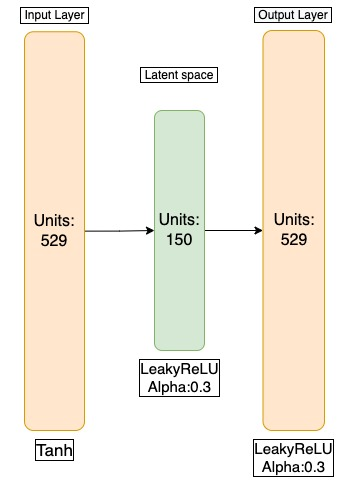
\includegraphics[scale=0.4]{Figures/nnarchitect/ae_small.jpeg}
    \caption[AE | Small network architecture]{Small autoencoder architecture.}
    \label{fig:ae_small}
\end{figure}

Figure \ref{fig:ae_small} shows the small autoencoder. It consists of an input and output layer of 529 nodes, with 
one latent space layer of 150 nodes. The activation functions for the input, latent space and output are the Tanh and 
LeakyReLU with $\alpha=0.3$ respectively.


\begin{figure}[H]
    \centering
    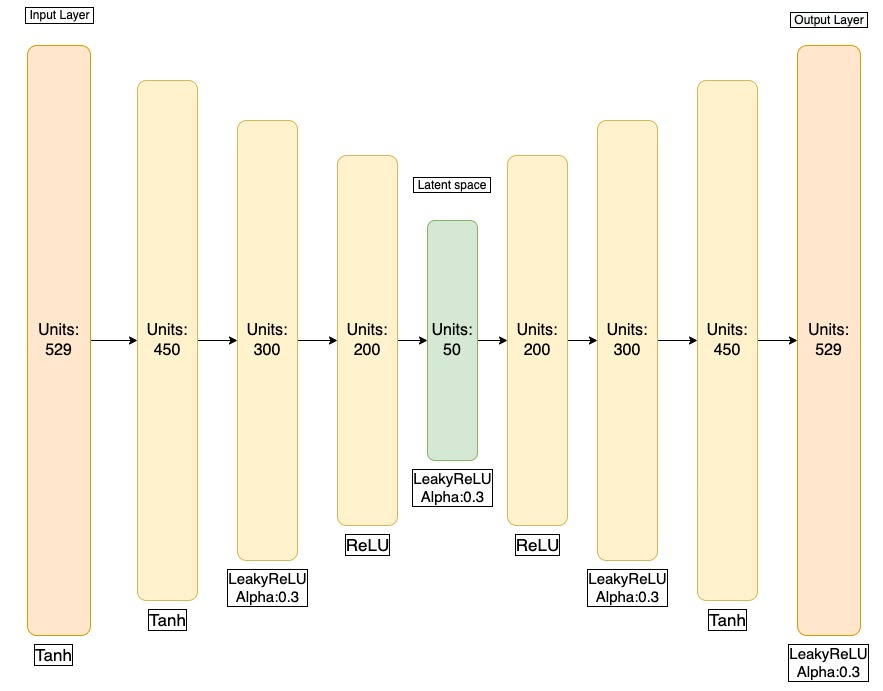
\includegraphics[width=0.8\textwidth]{Figures/nnarchitect/ae_big.jpeg}
    \caption[AE | Large network architecture]{Large autoencoder architecture.}
    \label{fig:ae_big}
\end{figure}

Figure \ref{fig:ae_big} shows the large autoencoder. It consists of an input and output layer of 529 nodes, with three 
hidden layers of 450, 300 and 200 nodes respectively in the encoder and three hidden layers of 200, 300 and 450 respectively. 
The activation functions for the input and ouput layers are the Tanh and LeakyReLU with $\alpha=0.3$ respectively. The hidden 
layers in the encoder have the activation functions Tanh, LeakyReLU with $\alpha=0.3$ and ReLU respectively. The hidden layers
in the decoder have the activation functions ReLU, LeakyReLU with $\alpha=0.3$ and Tanh respectively. The latent space has 150 nodes,
with the LeakyReLU activation function with $\alpha=0.3$.
\subsection*{The variational Autoencoder}
Below are the two models used for the variational autoencoder. 

\begin{figure}[H]
    \centering
    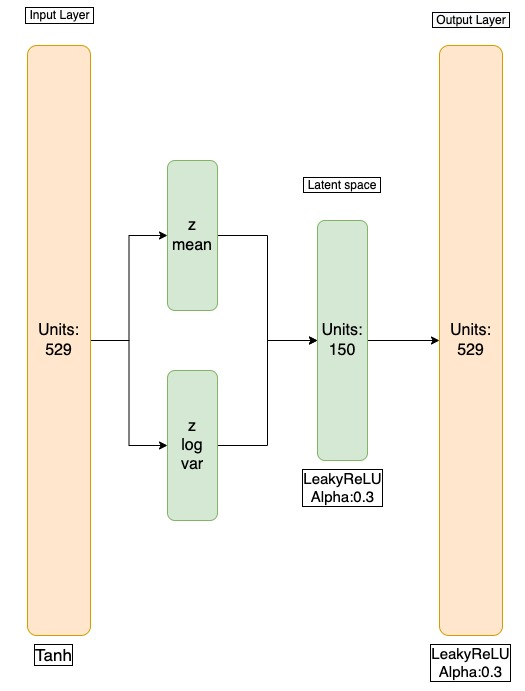
\includegraphics[scale=0.4]{Figures/nnarchitect/vae_small.jpeg}
    \caption[VAE | Small network architecture]{Small variational autoencoder architecture.}
    \label{fig:vae_small}
\end{figure}

In figure \ref{fig:vae_small} we have the small variational autoencoder. It consists of an input and output layer of 529 nodes, with 
one latent space layer of 150 nodes sampling from a mean and variance layer of same size. The activation functions for the input and 
output are the Tanh and LeakyReLU with $\alpha=0.3$ respectively.

\begin{figure}[H]
    \centering
    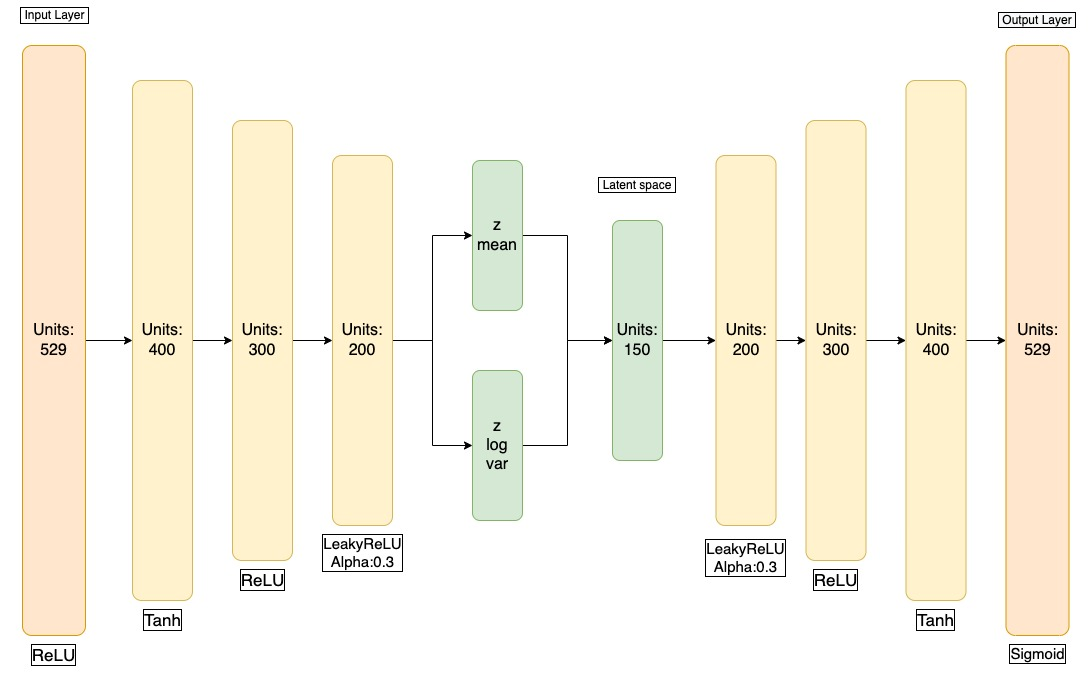
\includegraphics[width=0.8\textwidth]{Figures/nnarchitect/vae_big.jpeg}
    \caption{Large variational autoencoder architecture.}
    \label[VAE | Large network architecture]{fig:vae_big}
\end{figure}


In figure \ref{fig:vae_big} we have the large variational autoencoder. It consists of an input and output layer of 529 nodes, with three 
hidden layers of 400, 300 and 200 nodes respectively in the encoder and three hidden layers of 200, 300 and 400 respectively. 
The activation functions for the input and ouput layers are the ReLU and Sigmoid respectively. The hidden 
layers in the encoder have the activation functions Tanh, ReLU, LeakyReLU with $\alpha=0.3$ respectively. The hidden layers
in the decoder have the activation functions LeakyReLU with $\alpha=0.3$, ReLU and Tanh respectively.